% !TEX root = ../../Beamer/statikz/statikz.tex


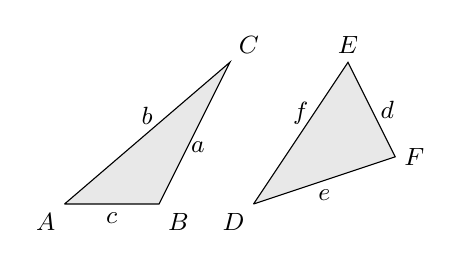
\begin{tikzpicture}[scale=0.6]

	\coordinate (A) at (0,0);
	\coordinate (B) at (2,0);
	\coordinate (C) at (3.5,3);
  \coordinate (D) at (4,0);
	\coordinate (E) at (6,3);
	\coordinate (F) at (7,1);

	\small
	\filldraw[fill=Gainsboro!65, draw=black] (A) -- node[below] {$c$}(B) --  node[below] { \;$a$}(C) --  node[above] {$b$} (A);
  \filldraw[fill=Gainsboro!65, draw=black] (D) -- node[above] {$f$}(E) --  node[right] {$d$}(F) --  node[below] {$e$} (D);

	\draw[below right] (B) node {$B$};
	\draw[below left] (A) node {$A$};
	\draw[above right] (C) node {$C$};
  \draw[below left] (D) node {$D$};
	\draw[above] (E) node {$E$};
	\draw[right] (F) node {$F$};

	% \node[xshift=-0.5cm, yshift=0.15cm] at (C) {$\theta $};



\end{tikzpicture}
